\documentclass{article}
\usepackage[utf8]{inputenc}
\usepackage{amsmath}
\usepackage{geometry}
\geometry{
 a4paper,
 total={182mm,257mm},
 left=14mm,
 top=20mm,
 }
 \usepackage[utf8]{inputenc}
 \usepackage[italian]{babel}
\usepackage[T1]{fontenc}
\usepackage{amssymb}
\usepackage{physics}
\usepackage{tikz}
\usepackage{graphicx}
\graphicspath{ {Immagini/Dinamica/} }
\usepackage{float}
\usepackage{hyperref}
\hypersetup{
    colorlinks=true,
    linkcolor=red,
    citecolor=green
    filecolor=magenta,      
    urlcolor=cyan,
}


%Theorem Environments
\newtheorem{thm}{Teorema}[section]
\newtheorem{lem}[thm]{Lemma}
\newtheorem{property}{Proprietà}[section]
\newtheorem{defn}{Definizione}[section]
\newtheorem{prop}[defn]{Proposizione}
\newtheorem{example}{Esempi}[subsection]
\newtheorem{exerc}[example]{Esercizi Svolti}

%Commandi di Formattazione
\newcommand{\noi}{\noindent}
\newcommand{\note}{\noindent {\quad \bf \underline{Osservazione:}} \quad}
\newcommand{\eg}{\noindent {\bf \underline{Esempio:}} \quad}
\newcommand{\bfemph}[1]{\textbf{\textit{#1}}}
\renewcommand{\emph}[1]{\bfemph{#1}}

%Number Sets
\newcommand{\R}{\mathbb{R}}
\newcommand{\C}{\mathbb{C}}
\newcommand{\Z}{\mathbb{Z}}
\newcommand{\Q}{\mathbb{Q}}

%Shortcuts
\newcommand{\then}{\ensuremath{\Rightarrow}}
\newcommand{\twopartdef}[4]
{
	\left\{
		\begin{array}{ll}
			#1 & \mbox{se } #2 \\
			#3 & \mbox{se } #4
		\end{array}
	\right.
}

%Vectors
\renewcommand{\i}{\vu{i}}
\renewcommand{\j}{\vu{j}}
\renewcommand{\k}{\vu{k}}
\renewcommand{\a}{\va{a}}
\renewcommand{\b}{\va{b}}
\renewcommand{\c}{\va{c}}
\renewcommand{\v}{\va{v}}
\renewcommand{\u}{\va{u}}
\newcommand{\s}{\va{s}}
\renewcommand{\t}{\va{t}}
\newcommand{\verst}{\vu{t}}
\newcommand{\versr}{\vu{r}}
\renewcommand{\r}{\va{r}}
\newcommand{\tauvs}{\vu{\tau}}
\newcommand{\tauvt}{\va{\tau}}
\newcommand{\normvs}{\vu{n}}
\newcommand{\N}{\va{N}}
\newcommand{\g}{\va{g}}
\newcommand{\F}{\va{F}}
\newcommand{\f}{\va{f}}
\newcommand{\p}{\va{p}}
\newcommand{\J}{\va{J}}




\title{Dinamica}
\author{Roberto Gargiulo}
\date{\today}

\begin{document}

\maketitle
\tableofcontents
\pagebreak


\section{Dinamica del Corpo Puntiforme}

\subsection{I Principi della Dinamica}

\subsubsection{I Principio}
Il I Principio è anche noto come \textbf{Principio d'Inerzia} e stabilisce:
\begin{defn}[Principio d'Inerzia]
Un corpo isolato (non soggetto a interazioni con altri corpi) non subisce cambiamenti di velocità. Se era in stato di quiete rimane in stato di quiete, se era in stato di moto si muove di moto rettilineo uniforme.
Può essere riformulato come segue:
\[ \dv{\s(t)}{t}=\v_0 \iff \dv[2]{\s(t)}{t}=0\]
\end{defn}



\subsubsection{II Principio}

Noto anche come \textbf{Legge di Newton} il II principio stabilisce:
\begin{defn}[Legge di Newton]
L'interazione di un punto materiale, espresso tramite la forza $\F$, determina l'accelerazione del punto proporzionalmente ad essa e alla \textbf{massa inerziale del corpo}. Può essere riformulato come segue:
\[\F=m\a=m\dv[2]{\s(t)}{t}\]
\end{defn}

\begin{prop}[Massa Inerziale]
Per quanto stabilito dai primi due principi della dinamica ogni corpo presenta una tendenza, l'\textbf{inerzia}, a opporsi alla variazione di moto, possiamo quantificare tale tendenza e la chiamiamo \textbf{massa inerziale}.\\
Operativamente, noto il valore di una certa forza $\F$ e scelto un certo campione $m_0$ possiamo stabilire un'unità di misura per la massa inerziale misurando il rapporto tra le accelerazioni (e di conseguenza le accelerazioni stesse) dovute alla forza $\F$ applicata ai due corpi:
\[\F=m_0\a_0=m\a\then m=m_0\frac{|\a|}{|\a_0|}\]
\end{prop}


\subsubsection{III Principio}
Noto anche come \textbf{Principio di Azione e Reazione} esso stabilisce:
\begin{defn}
Se un corpo A esercita una certa forza $\F_{A\to B}$ su un altro corpo B, allora tale corpo esercita una forza uguale e opposta sul corpo A che agisce sulla stessa direzione della prima tale che entrambe abbiano verso diretto da un corpo verso l'altro. Otteniamo quindi:
\begin{equation}
\label{interazioniopposte}
\F_{A\to B}=-\F_{B\to A}
\end{equation}
Inoltre dato un certo sistema di riferimento:
\begin{equation}
\label{direzioneinter}
\left\{\begin{array}{l}
    (\r_1-\r_2)\parallel \F_{B\to A}  \\
    (\r_2-\r_1)\parallel \F_{A\to B}  \\ 
\end{array}\right.\then
\left\{\begin{array}{l}
    (\r_1-\r_2)\times\F_{B\to A}=0  \\
    (\r_2-\r_1)\times\F_{A\to B}=0  \\ 
\end{array}\right.
\end{equation}
Combinando la \ref{interazioniopposte},\ref{direzioneinter} e il II Principio otteniamo quindi la seguente formulazione del terzo principio per un sistema di corpi:
\begin{equation}
    \sum_{i,j=1}^n \r_i\times(m_j\a_j)=0
\end{equation}
\end{defn}

\subsection{Le Reazioni Vincolari}

\begin{defn}
\textbf{Vincolo} Una qualsiasi condizione che limita il moto di un corpo e che può essere espressa da una certa equazione/disuguaglianza relativa ad una funzione $f(\r,\v,\a,t)$ del corpo.
\end{defn}

\begin{defn}
\textbf{Vincolo Olonomo} Vincolo che dipende da posizione e tempo, in particolare del tipo: \(f(\r,t)=0\)
\end{defn}
\begin{defn}
\textbf{Vincolo Anolonomo} Vincolo che dipende anche dalla velocità, oltre che tempo e posizione: \(f(\r,\v,t)=0\)
\end{defn}

\begin{example}
\begin{enumerate}
    \item Consideriamo il caso di un corpo che si muove di moto circolare, esprimendo il vincolo come segue:
    \[f(x,y)=x^2(t)+y^2(t)-R=0\]
    Dove si sceglie il riferimento che abbia origine nel centro della circonferenza, la quale ha raggio R.
    \item Il vincolo di un piano inclinato è invece dato da:
    \[\frac{z(t)}{x(t)}=\tan\alpha\]
    Dove si sceglie il riferimento i cui due assi sono uno orizzontale e l'altro verticale uscente dal suolo.
\end{enumerate}
\end{example}


\note Ovviamente notiamo che scegliendo diversi sistemi di riferimento cambiano anche le espressioni dei vincoli, ad esempio nel caso del piano inclinato scegliendo un sistema di riferimento un cui asse coincide con il piano inclinato significa porre:
\[f(x)=x(t)=0\]

\begin{defn}
\textbf{Gradi di Libertà} di un Punto Materiale sono $dimV_3-N^\circ$Vincoli, che indicano in quanti "modi" si può muovere un corpo.
\end{defn}

\begin{prop}[Macchina di Atwood]
La Macchina di Atwood è una macchina composta dalla tipica carrucola ai cui lati sono appesi due corpi.

\begin{figure}[H]
    \centering
    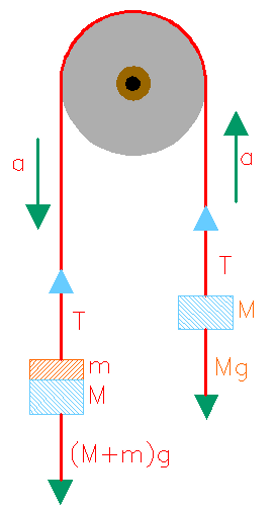
\includegraphics[width=0.25\textwidth]{0650_d1.png}
    \caption{Macchina di Atwood}
    \label{atwoodmachine}
\end{figure}

Dove i corpi hanno massa $m_1,m_2$ rispettivamente e quota $z_1,z_2$ rispettivamente in un riferimento cartesiano centrato nella carrucola (da considerarsi puntiforme) con un asse parallelo al filo e diretto verso il basso. Allora il vincolo della macchina può essere inteso come la lunghezza costante del filo e si può esprimere come segue:
\[f(z)=z_1(t)+z_2(t)-l=0\]
Da cui otteniamo un vincolo per le accelerazioni:
\[\dv[2]{z_1}{t}+\dv[2]{z_2}{t}=0\]
Inoltre per il II principio (posto per comodità $m_2>m_1$ in modo che $a_1<0$):
\[m_1g-|\va{\tau}|=-m_1a_1\quad m_2g-|\va{\tau}|=m_2a_2\]
Otteniamo allora il seguente sistema:
\[\left\{\begin{array}{l}
    a_1(t)+a_2(t)=0  \\
    |\a_1(t)|=a=-g+\frac{|\va{\tau}|}{m_1}\\
    |\a_2(t)|=g-\frac{|\va{\tau}|}{m_2}
\end{array}\right.\]
E quindi l'\textbf{equazione vincolare rispetto alla tensione}:
\begin{equation}
    \boxed{|\va{\tau}|=2g(m_1+m_2)}
\end{equation}
\end{prop}

\begin{prop}
Consideriamo una Macchina composta da due carrucole collegate da un unico filo, una delle quali è mobile ed ha massa non trascurabile, come in figura: 
\begin{figure}[H]
    \centering
    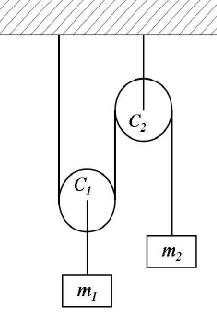
\includegraphics[width=0.25\textwidth]{2i8g76b.png}
    \caption{Carrucola Composta da una mobile e una fissa}
    \label{carrucolamobile}
\end{figure}

Dette $m_1,m_2,m_c$ le masse dei due corpi e della carrucola mobile rispettivamente, allora il vincolo della lunghezza del filo è dato dal sistema:
\[\left\{\begin{array}{l}
    z_2-z_c-l_1=0  \\
    2z_c+z_1-l_2=0 
\end{array}\right.\]
Derivando due volte entrambe le equazioni otteniamo quindi:
\[\left\{\begin{array}{l}
    z_2''(t)-z_c''(t)=0  \\
    2z_c+z_1-l_2=0 
\end{array}\right.\]
\end{prop}


\section{Leggi di Forze}

\subsection{Introduzione}
Tutte forze possono esprimersi come funzioni di $\r,\v,\a,t$ e più in particolare $\r,t$.

\subsection{Forze Notevoli}

\begin{defn}
\textbf{Forza Peso/Forza Gravitazionale}:
\begin{enumerate}
    \item Simbolo: $\va{P}$
    \item Modulo: $m\cdot g$
    \item Direzione: Parallelo al vettore posizione nel sistema di riferimento centrato nel centro della Terra ("verticalre)
    \item Verso: Dal corpo al centro della Terra
    \item Note Ulteriori: \(\va{P}=-G\frac{M_Tm}{r^2}\vu{r}=m\va{g}\)
\end{enumerate}
\end{defn}
\begin{prop}[Legge della Forza di Gravità]
Dati i corpi di masse gravitazionali $m_1,m_2$ e raggi vettori $\r_1,\r_2$ in un certo riferimento allora l'interazione gravitazionale tra il corpo 1 e il corpo 2 è:
\[\f_{12}=G\frac{m_1m_2}{|\r_2-\r_1|^1}\vu{r}_{21}=G\frac{m_1m_2}{|\r_2-\r_1|^2}\frac{(\r_2-\r_1}{|\r_2-\r_1|}=G\frac{m_1m_2}{|\r_2-\r_1|^3}(\r_2-\r_1)=m_1\dv[2]{\r_1}{t}\]
(Per il II Principio).\\
Similmente l'interazione tra il corpo 2 e il corpo 1:
\[\f_{21}=G\frac{m_1m_2}{|\r_1-\r_2|^3}(\r_1-\r_2)=m_2\dv{\r_2}{t}\]
\end{prop}


\begin{defn}
\textbf{Reazione Vincolare Normale}:
\begin{enumerate}
    \item Simbolo: $\va{N}$
    \item Modulo: Dipende dalla condizioni di equilibrio
    \item Direzione: Perpendicolare alla superficie di contatto
    \item Verso: Si oppone alla compenetrazione dei corpi
\end{enumerate}
\end{defn}
\begin{prop}
Quando un punto materiale interagisce con un corpo dalla superficie curva, allora la direzione della forza è sempre perpendicolare alla superficie, stavolta però non è costante.
\end{prop}

\begin{defn}
\textbf{Forza d'Attrito Statica}:
\begin{enumerate}
    \item Simbolo: $\va{f}_a$
    \item Modulo: Dipende dalle condizioni di equilibrio
    \item Direzione: Tangente alla superficie di contatto
    \item Verso: //
\end{enumerate}
\end{defn}
\begin{property}
La Forza d'Attrito Radente si può presentare sotto due regimi:
\begin{enumerate}
    \item \textbf{Regime Statico} in cui la forza d'attrito eguaglia la forza "spingente" e il quale si supera raggiunta una certa forza $\mu_S|\N|$ dove $\mu_S$ è detto \textbf{coefficiente d'attrito statico}.
    \item \textbf{Regime Dinamico} in cui la forza d'attrito ha valore costante $\mu_d|\N|<\mu_S|\N|$ dove $\mu_d$ è detto \textbf{coefficiente d'attrito dinamico}.
\end{enumerate}
Nel caso di un corpo in regime dinamico (ad esempio in discesa lungo un piano inclinato) possiamo determinare le leggi oraria di posizione, velocità e accelerazione a partire dalla risultante delle forze (scelto un sistema di riferimento centrato nella posizione iniziale del corpo, un asse rivolto verso il basso e parallelo al piano, l'altro perpendicolare e uscente):
\[\j) |\N|-mg\cos\alpha=0\iff |\N|=mg\cos\alpha\]
\[\i) mg\sin\alpha-\mu_dmg\cos\alpha=ma\iff a=g(\sin\alpha-\mu_d\cos\alpha)\]
Posto $\lambda^\pm=(\sin\alpha\pm\mu_d\cos\alpha)$ allora le leggi oraria sono le seguenti (con velocità iniziale $v_0$ e istante iniziale $t_0$):
\[\left\{\begin{array}{l}
    x(t)=v_0(t-t_0)-\frac{g\lambda^-}{2}(t-t_0)^2   \\
    v(t)=v_0+g\lambda^-(t-t_0)    \\
    a(t)=g\lambda^-   \\
\end{array}\right.\]
\end{property}



\begin{defn}
\textbf{Tensione di un Filo/Sbarra Ideale}:
\begin{enumerate}
    \item Simbolo: $\va{\tau}$
    \item Modulo: Dipende dalle condizioni di equilibrio
    \item Direzione: Parallela a quella del filo
    \item Verso: Dal corpo al supporto
    \item Note Ulteriori: Un filo ideale si può considerare come un filo composto da infinitesime parti a cui viene applicata una forza dalla precedente e che applicano la stessa forza alla parte successiva, trasmettendo perfettamente la forza dal sostegno al corpo appeso.
\end{enumerate}
\end{defn}


\begin{defn}
\textbf{Forza Elastica}:
\begin{enumerate}
    \item Simbolo: $\va{F}_e$
    \item Modulo: $k\delta l$
    \item Direzione: Parallela all'asse della molla
    \item Verso: Opposto alla deformazione
\end{enumerate}
\end{defn}

\section{Conseguenze dei Principi della Dinamica}

\subsection{Quantità di Moto e Impulso}

\begin{defn}
\textbf{Quantità di Moto} \(\p=m\v\)
\end{defn}
\note \hypertarget{quantità-forza}{Se la massa è costante allora si ottiene}:
\[\dv{\p}{t}=\dv{(m\v)}{t}=m\dv{\v}{t}=m\a=\F\]
Che è una versione più generale del II Principio anche per masse non costanti, tale che possiamo intendere l'interazione di due corpi come una variazione della velocità (in modulo, direzione, verso) oppure la sua massa.

\begin{thm}[Teorema dell'Impulso]
\label{teoremaimpulso}
Detto $\J$ il vettore ottenuto integrando una forza $\F$ applicato in un intervallo di tempo $t$, che chiamiamo \textbf{Impulso della Forza}:
\[\J=\int_0^t\F \dd t\]
Per quanto \hyperlink{quantità-forza}{notato} otteniamo:
\[\J=\int_0^t\F \dd t=\int_0^t\dv{\p}{t} \dd t=\int_{\p_0}^{\p}\dd \p=\p-\p_0=\Delta \p\then \boxed{\J=\Delta\p}\]
Ossia l'applicazione di una forza ad un corpo per un certo intervallo di tempo causa una variazione della quantità di moto.
\end{thm}
\note Se la massa è costante il Teorema dell'Impulso si riduce a:
\[\J=m(\v-v_0)=m\Delta\v\]
Inoltre usando il Teorema della Media Integrale possiamo calcolare il valore medio della forza nota la variazione di quantità di moto:
\[\F_m=\frac{\Delta\p}{t}\]

\begin{prop}[Conservazione della Quantità di Moto]
Diretta conseguenza del Teorema dell'Impulso è che se la risultante delle forze applicate ad un sistema è nulla, allora la quantità di moto si conserva. Per corpi di massa costante tale principio è solo un'estensione del Principio d'Inerzia.
\end{prop}

\subsection{Urti}
\begin{defn}
Un'interazione tra due o più corpi che abbia durata limitata.
\end{defn}

\begin{prop}
Studiare un urto significa misurare le quantità di moto iniziali e finali dei corpi coinvolti. Inoltre, per la Conservazione della Quantità di Moto la variazione totale di quantità di moto è nulla:
\[\Delta\p_1+\Delta\p_2=(\p'_1-\p_1)+(\p'_2-\p_2)=0\]
\end{prop}

\begin{example}
Un esempio di urto tra due corpi può essere anche l'avvicinamento di un asteroide al sole. Tuttavia in una gran parte delle considerazioni relative agli urti si considera che lo spostamento e la durata dell'urto siano entrambe nulle (infinitesime).
\end{example}


\end{document}